\documentclass[10pt, a4paper]{article}

%%% SST LAB PROTOCOLL PREAMBLE
%%% 2019
%%%%%%%%%%%%%%%%%%%%%%%%%%%%%%%


%%% PACKAGES
%%%%%%%%%%%%%%%%%%%%%%%%%%%

\usepackage[ngerman]{babel}

\usepackage[utf8]{inputenc}
\usepackage{amsmath}
\usepackage{pgfplots}
\usepackage{tikz}
\usepackage[many]{tcolorbox}
\usepackage{graphicx}
\graphicspath{ {./graphics/} }
\usepackage{pdfpages}
\usepackage{dashrule}
\usepackage{float}
\usepackage{siunitx}
\usepackage{trfsigns}
\usepackage{booktabs}
\usepackage[european]{circuitikz}
\usepackage{tcolorbox}

%%% DOCUMENT GEOMETRY
%%%%%%%%%%%%%%%%%%%%%%%%%%%

\usepackage{geometry}
\geometry{
 a4paper,
 total={0.6180339887498948\paperwidth,0.6180339887498948\paperheight},
 top = 0.1458980337503154\paperheight,
 bottom = 0.1458980337503154\paperheight
 }
\setlength{\jot}{0.013155617496424828\paperheight}
\linespread{1.1458980337503154}

\setlength{\parskip}{0.013155617496424828\paperheight} % paragraph spacing


%%% COLORS
%%%%%%%%%%%%%%%%%%%%%%%%%%%

\definecolor{red1}{HTML}{f38181}
\definecolor{yellow1}{HTML}{fce38a}
\definecolor{green1}{HTML}{95e1d3}
\definecolor{blue1}{HTML}{66bfbf}
\definecolor{hsblue}{HTML}{00b1db}
\definecolor{hsgrey}{HTML}{afafaf}

%%% CONSTANTS
%%%%%%%%%%%%%%%%%%%%%%%%%%%
\newlength{\smallvert}
\setlength{\smallvert}{0.0131556\paperheight}


%%% COMMANDS
%%%%%%%%%%%%%%%%%%%%%%%%%%%

% differential d
\newcommand*\dif{\mathop{}\!\mathrm{d}}

% horizontal line
\newcommand{\holine}[1]{
  	\begin{center}
	  	\noindent{\color{hsgrey}\hdashrule[0ex]{#1}{1pt}{3mm}}\\%[0.0131556\paperheight]
  	\end{center}
}

% mini section
\newcommand{\minisec}[1]{ \noindent\underline{\textit {#1} } \\}

% quick function plot
\newcommand{\plotfun}[3]{
  \vspace{0.021286\paperheight}
  \begin{center}
    \begin{tikzpicture}
      \begin{axis}[
        axis x line=center,
        axis y line=center,
        ]
        \addplot[draw=red1][domain=#2:#3]{#1};
      \end{axis}
    \end{tikzpicture}
  \end{center}
}

% box for notes
\newcommand{\notebox}[1]{

\tcbset{colback=white,colframe=green1!100!black,title=Note!,width=0.618\paperwidth,arc=0pt}

 \begin{center}
  \begin{tcolorbox}[]
   #1 
  \end{tcolorbox}
 
 \end{center} 
 
}

% box for equation
\newcommand{\eqbox}[2]{
	
	\tcbset{colback=white,colframe=green1!100!black,title=,width=#2,arc=0pt}
	
	\begin{center}
		\begin{tcolorbox}[ams align*]
				#1
		\end{tcolorbox}
		
	\end{center} 
	
}
% END OF PREAMBLE
\newcommand{\upperRomannumeral}[1]{\uppercase\expandafter{\romannumeral#1}}
\newtcbox{\inlinecodee}{on line, boxrule=0pt, boxsep=0pt, top=2pt, left=2pt, bottom=2pt, right=2pt, colback=gray-2, colframe=white, fontupper={\ttfamily \footnotesize}}

\begin{document}

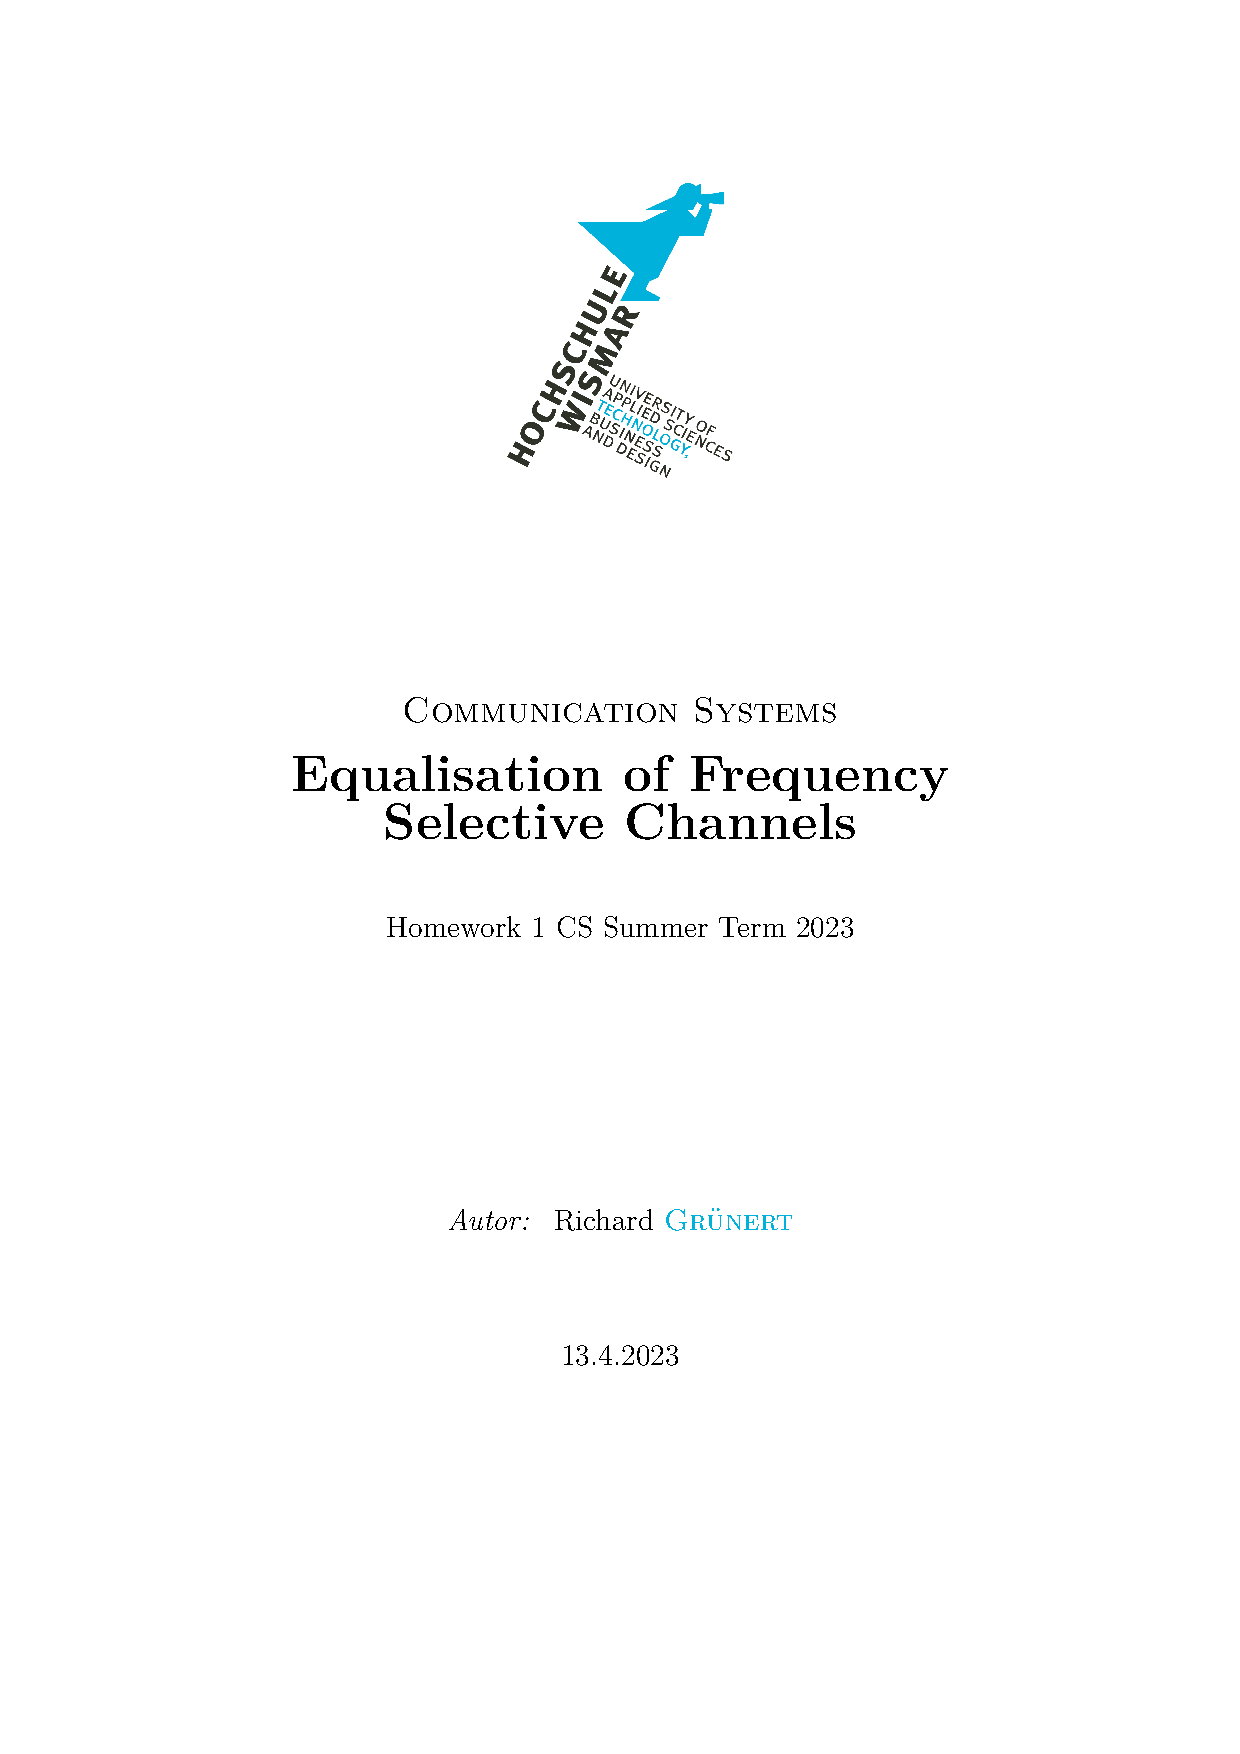
\includepdf{./titlepage/titlepage.pdf}

\section{Procedure / Method}
Using \textsc{Matlab Simulink}\texttrademark{}, the provided model file \inlinecodee{M5\_T\_EQL\_FIR\_pre.slx} as well as the \inlinecodee{initial\_.m} file have been extended to include an additional equalizer at the receiver side. Figure \ref{fig:system_screenshot} shows a screenshot of the model in Simulink.\\

\begin{figure}[H]
\centering
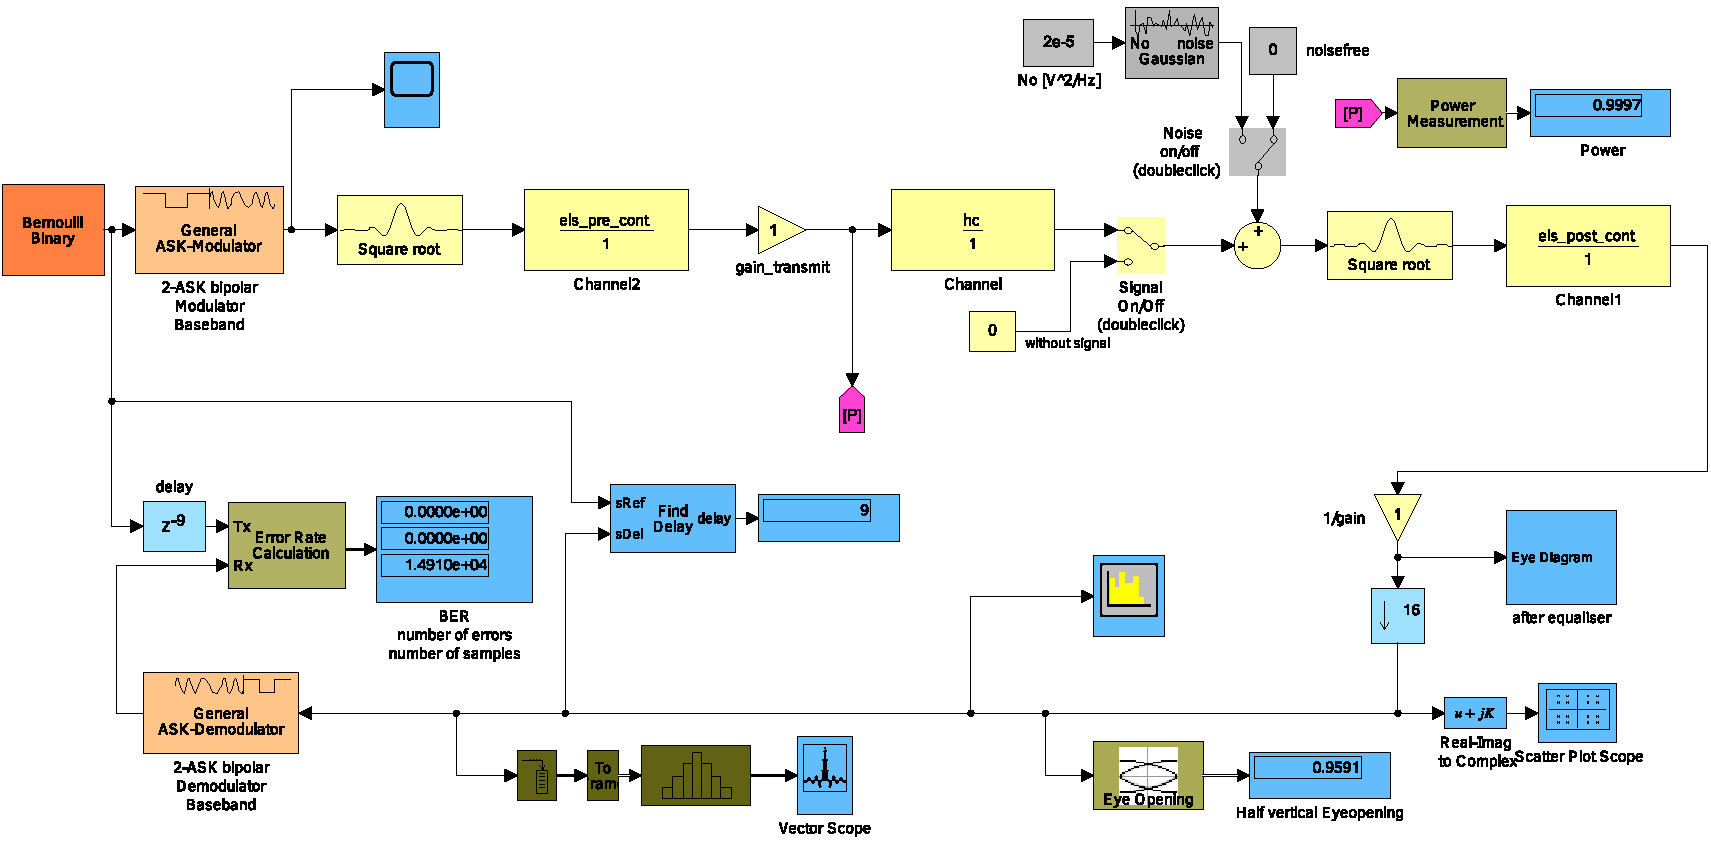
\includegraphics[width=0.764\textwidth]{graphics/system_screenshot.pdf}
\caption{Simulation System}\label{fig:system_screenshot}
\end{figure}

Either of the equalizers can be put into ``thru''-mode by setting the coefficients of the respective FIR-Block to \inlinecodee{[ 1 0 0 ... 0 0 0 ]}. The equalization was done using $5$ coefficients.

\section{Model Check}

The AWGN conditions with a non-frequency-selective channel have been checked and without any noise addition, the two symbols were clearly distinguishable, as expected.\\

With the simulated power measurement, the signal power shows $P_{s} = 1\, \si{\volt\squared}$. Multiplying by the symbol time $T_{sym} = \frac{1}{5000}\,\si{\second} = 2\cdot 10^{-4}\,\si{\second}$, gives a symbol energy of $E_{s} = 2\cdot 10^{-4}\,\si{\volt\squared\second}$. With the set noise power density of $N_{0} = 2\cdot 10^{-5}\,\si{\volt\squared\per\hertz}$, the channel SNR becomes

\[
  \frac{E_{s}}{N_{0}} = \frac{2\cdot 10^{-4}\,\si{\volt\squared\second}}{2\cdot 10^{-5}\,\si{\volt\squared\per\hertz}} = 10 \rightarrow 10 \,\si{\deci\bel}
\]

as required.


\subsection{Procedure for each Channel Type}
With the provided spreadsheet, each channel type could be characterised. The best nyquist vector for each situation was noted.\\

The simulation time was $30\,\si{\second}$ in each case. The simulation results can be found in Table \ref{tab:sim_results} as well as in the accompanying spreadsheet. The modified simulation model and Matlab script file are also attached.


\section{Channel \upperRomannumeral{1}: 2-Tap Minimum Phase Channel}


\subsection{Difference between calculated and simulated BER}\label{sec:ber_calc_sim_diff}
In the case of not using any equalizer, one finds that the BER resulting from the simulation is approximately half of that which was calculated.\\

This is due to the fact that the ISI introduced by the channel causes four possible signal values to appear at the sampling point (without any noise influence). This can be easily seen in the eye diagram in Figure \ref{fig:min_phase_eye_no_noise}.\\

In this case, a sent symbol (1 or 0 in this case) could be moved by the ISI to have a magnitude of $0.45$ or $1.35$. $50\,\si{\percent}$ of the sent symbols will be received as either $0.45$ or $-0.45$ and the other $50\,\si{\percent}$ will be either $1.35$ or $-1.35$.\\

Since the symbols with the greater magnitude ($1.35$) will have a greater $U_{A}$ their error probability will be lower under the infuence of noise, given the same noise power. We get two different error probabilities:
\[P_{e1} = \frac{1}{2} \cdot \textrm{erfc}{\left(\frac{\color{red-5}{0.45\,\si{\volt}}}{\sqrt{2}\cdot\sqrt{0.1\,\si{\volt\squared}}}\right)} = 7.7\cdot 10^{-2}\]
\[P_{e2} = \frac{1}{2} \cdot \textrm{erfc}{\left(\frac{\color{red-5}{1.35\,\si{\volt}}}{\sqrt{2}\cdot\sqrt{0.1\,\si{\volt\squared}}}\right)} = 1.1\cdot10^{-5}\]

i.e. the symbols with magnitude $1.35$ will be less likely to cause errors. Given that the error probability is much lower for the higher-magnitude symbols, their errors can be neglected. This means that $50\,\si{\percent}$ of the symbols will not cause any errors which explains that the calculated BER is approximately two times as large as the simulated BER since the equation does not model this ISI-behaviour.

The total error rate is:
\[P_{e} = 0.5 \cdot P_{e1} + 0.5 \cdot P_{e2} = 0.5\cdot 7.7011 \cdot 10^{-2} \approx 3.9 \cdot 10^{-2}\]

which matches the simulated value $4.0\cdot 10^{-2}$ well.

\begin{figure}%[H]
\centering
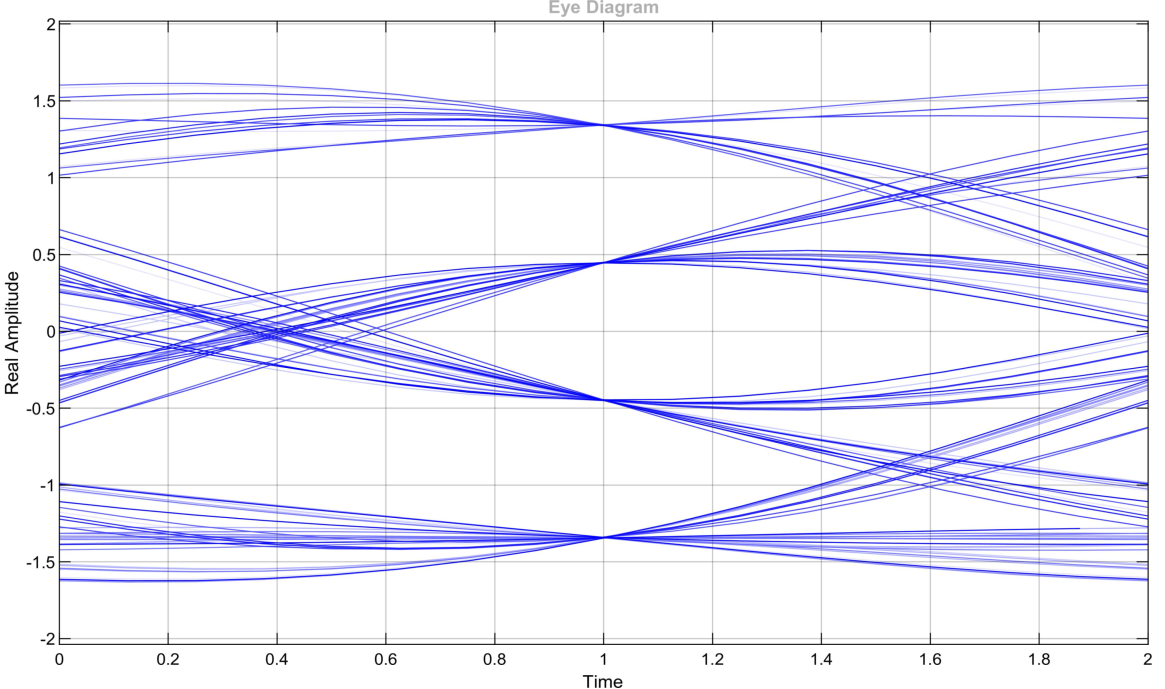
\includegraphics[width=0.764\textwidth]{graphics/eye_two_tap_min_phase_no_noise.pdf}
\caption{Eye diagram of system with two-tap minimum phase channel without noise.}\label{fig:min_phase_eye_no_noise}
\end{figure}


\subsection{Equalization}

\begin{figure}%[H]
\centering
\includegraphics[width=0.764\textwidth]{graphics/eye_two_tap_min_phase_no_noise_equalized.pdf}
\caption{Eye of equalized two-tap channel system (post-coding).}\label{fig:min_phase_eye_no_noise_equalized}
\end{figure}

Using the equalizer yields a lowered BER, as expected. The equalization is not perfect, however, as only a finite number of coefficients can be used. Figure \ref{fig:min_phase_eye_no_noise_equalized} shows the eye diagram and the remaining spread of values at the sample point which causes a lower $U_{A}$ than under AWGN conditions.

The simulated BER is also smaller than the calculated one. This can be explained by the fact that the calculation uses the minimal half vertical eye opening. However, as seen in Figure \ref{fig:min_phase_eye_no_noise_equalized} there exist also symbol amplitudes greater than this value causing the actual BER to be smaller. The highest of these is approximately $U_{A_{\text{max}}} = 1.05\,\si{\volt}$ resulting in a BER of

\[P_{e_{\text{min}}} = 5.4\cdot 10^{-3}\]

while the highest using the minimal eye opening is

\[P_{e_{\text{max}}} = 9.9\cdot 10^{-3}\]

so that the actual BER has to be in the interval $[P_{e_{\text{min}}}, P_{e_{\text{max}}}]$, which is the case ($P_{e_{\text{sim}}} = 7.3\cdot 10^{-3}$).

\subsubsection{Post- vs Pre-Coding}
In the post-coding case, the noise path will receive an increase in power by the greater-than-unity gain of the equalizer. The power gain can be calculated by taking the sum of the squared coefficients and is $G_{\text{EQ}} = 1.654$ so that the noise power after the equalizer will be $P_{\text{n}_{\text{calc}}} = 0.1654 \,\si{\volt\squared}$. This matches the measurement from the simulation ($P_{\text{n}_{\text{sim}}} = 0.17\,\si{\volt\squared}$).\\

By moving the equalizer to the sender side, it cannot increase the noise power as it is not part of the noise path. This is reflected in the BER simulation / measurement. This way, the BER could be improved by a factor of approximately $50$ compared to the case without any equalizer and is only slightly higher than the AWGN BER.


\section{Channel \upperRomannumeral{2}: 2-Tap Maximum Phase Channel}
\begin{figure}%[H]
\centering
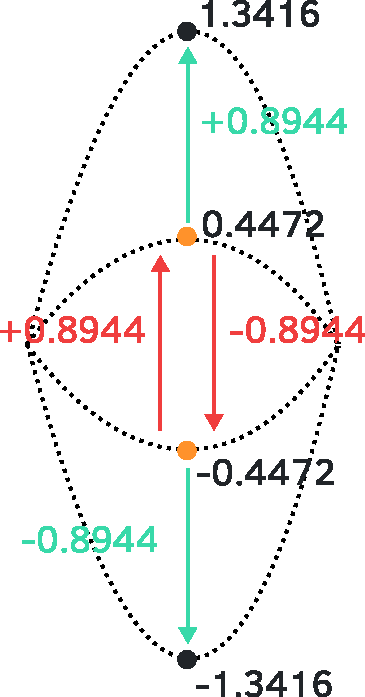
\includegraphics[height=0.3\textheight]{graphics/max_phase_eye_explanation.pdf}
\caption{Illustration of how the max-phase eye comes about. The orange points are the starting positions. The red arrows show the ISI-influences that cause bit errors. $\frac{1}{\sqrt{5}}\approx 0.4472$, $\frac{2}{\sqrt{5}}\approx 0.8944$.}\label{fig:two_tap_max_phase_illustration}
\end{figure}

For the maximum phase channel, the second channel coefficient (previous symbol) is larger than the first (current symbol). This results in an eye diagram as illustrated in figure \ref{fig:two_tap_max_phase_illustration}. Starting from the two possible reduced positions ($1\,\si{\volt}\cdot h_{0} = 0.4472\,\si{\volt}$), the influence of the previous symbol can be $1\,\si{\volt}\cdot h_{1} = +0.8944\,\si{\volt}$ or $-1\,\si{\volt}\cdot h_{1} = -0.8944\,\si{\volt}$. Two problematic situations arise:
\begin{enumerate}
        \item After a symbol with an amplitude of $-1\,\si{\volt}$, a symbol of amplitude $1\,\si{\volt}$ is sent
        \item After a symbol with an amplitude of $1\,\si{\volt}$, a symbol of amplitude $-1\,\si{\volt}$ is sent
\end{enumerate}

The first situation results in a received amplitude of

$$\underbrace{1\,\si{\volt} \cdot 0.4472}_{\text{current symbol}} + \underbrace{-1\,\si{\volt}\cdot 0.8944}_{\text{previous symbol}} = -0.4472\,\si{\volt}$$

even though a symbol with an amplitude of $1\,\si{\volt}$ has been sent. Similarly, the second situation results in

$$\underbrace{-1\,\si{\volt} \cdot 0.4472}_{\text{current symbol}} + \underbrace{1\,\si{\volt}\cdot 0.8944}_{\text{previous symbol}} = 0.4472\,\si{\volt}$$

even though a symbol with an amplitude of $-1\,\si{\volt}$ has been sent. So for these two situations, errors arise because the symbol amplitudes moved over the detector threshold. Assuming a uniformly distributed set of sent symbols, these error inducing transitions occur for $50\,\si{\percent}$ of all sent symbols. So a BER of $0.5$ is to be expected. The BER measurement from the simulation confirms this.\\

Using equalization does not help in this case. The BER stays at $0.5$. Whether post- or pre-coding is used does not matter, as $0.5$ is already the worst case. One explanation why this channel type is not equalizable can be seen by looking at the eye diagram. The eye diagram of this channel actually looks identical to the one from the minimum phase channel (see Figure \ref{fig:min_phase_eye_no_noise}). This means that from the receiver's point of view, it is impossible to distinguish between these two situations to develop an equalizer using the inverse-method. One way to solve this problem is to introduce additional delay at the receiver side.\\

%Since the amplitudes of $0.4472\,\si{\volt}$ and $-0.4472\,\si{\volt}$ always represent erroneous transmissions in this channel example, one could ``switch'' their mappings, thereby creating a sort of 4-ASK. %However, with the addition of noise, this would not work.

%Equalization using the inverse-method, i.e. finding a discrete impulse response $f(k)$ such that the channel's impulse reponse $h(k)$ convolved with it will result in a dirac impulse $\delta(k)$, does not work for nonminimum phase channels since it produces either a noncausal or unstable total response. Using a delay can solve this problem. \cite{radlovic_audio_eq}

\section{Channel \upperRomannumeral{2}: 3-Tap Mixed Phase Channel}

\begin{figure}%[H]
\centering
\includegraphics[width=0.764\textwidth]{graphics/eye_two_tap_mixed_phase_no_noise.pdf}
\caption{Eye of two-tap mixed phase channel system (no noise).}\label{fig:mixed_phase_eye_no_noise}
\end{figure}

\begin{figure}%[H]
\centering
\includegraphics[width=0.764\textwidth]{graphics/eye_two_tap_mixed_phase_no_noise_annotated.pdf}
\caption{Annotated eye of mixed phase channel. Values that are erroneous are colored in red.}\label{fig:mixed_phase_eye_no_noise_annotated}
\end{figure}


The channel mechanism is similar to the previous one. The additional influence of the symbol previous to the previous one leads the eye to have additional discrete values, see Figure \ref{fig:mixed_phase_eye_no_noise}. In this case, the eye opening is really small. Figure \ref{fig:mixed_phase_eye_no_noise_annotated} shows the possible symbol amplitude levels. Again, $50\,\si{\percent}$ of them are erroneous, leading to a BER of $0.5$.

Again, the inverse / zero-forcing strategy of equalization is insufficient in this case and another solution would have to be found.

The best vector of the nyquist conditions that minimizes the sum of the squared differences of the filter coefficients to itself is
\[z_{1} = [ 0, 1, 0, 0, 0, 0, 0 ]\]

while the best vector that minimizes the simulated BER is
\[z_{2} = [ 1, 0, 0, 0, 0, 0, 0 ]\]
with equalizer coefficients
\[f_{2} = [ 1.2948, -1.5365, 1.2833, -0.8282, 0.3486 ]\]
which results in a BER of $0.25$.

% Please add the following required packages to your document preamble:
% \usepackage[table,xcdraw]{xcolor}
% If you use beamer only pass "xcolor=table" option, i.e. \documentclass[xcolor=table]{beamer}
\begin{sidewaystable}[]
\begin{tabular}{llllllllll}
\rowcolor{gray-2}
Channel                      & Equalisation & $U_{a} / \si{\volt}$ & $U_{a}^2 / \si{\volt\squared}$ & $P_N / \si{\volt}$ & $\rho$ & BERcalc & BERSim  & Nyquist Vector        & EQ Coefficients                                  \\
\rowcolor{yellow-1}
AWGN                         & -            & 1                    & 1                              & 0.1                & 10     & 7.8E-04 & 8.1E-04 & -                     & -                                                \\
\rowcolor{green-1}
{[} 2/sqrt(5), 1/sqrt(5) {]} & none         & 0.45                 & 0.2025                         & 0.1                & 2.025  & 7.7E-02 & 4.0E-02 & -                     & -                                                \\
\rowcolor{green-1}
                             & post         & 0.96                 & 0.9216                         & 0.17               & 5.421  & 9.9E-03 & 7.3E-03 & {[} 1 0 0 0 0 0 0 {]} & {[} 1.1172, -0.5570, 0.2752, -0.1311, 0.0524 {]} \\
\rowcolor{green-1}
                             & pre          & 0.96                 & 0.9216                         & 0.1                & 9.216  & 1.2E-03 & 8.5E-04 & {[} 1 0 0 0 0 0 0 {]} & {[} 1.1172, -0.5570, 0.2752, -0.1311, 0.0524 {]} \\
\rowcolor{blue-1}
{[} 1/sqrt(5), 2/sqrt(5) {]} & none         & 0.44                 & 0.1936                         & 0.1                & 1.936  & 8.2E-02 & 4.6E-01 & -                     & -                                                \\
\rowcolor{blue-1}
                             & post         & 0.96                 & 0.9216                         & 0.17               & 5.421  & 9.9E-03 & 5.0E-01 & {[} 0 0 0 0 0 1 0 {]} & {[} 0.0524 -0.1311 0.2752 -0.5570 1.1172 {]}     \\
\rowcolor{blue-1}
                             & pre          & 0.96                 & 0.9216                         & 0.1                & 9.216  & 1.2E-03 & 5.0E-01 & {[} 0 0 0 0 0 1 0 {]} & {[} 0.0524 -0.1311 0.2752 -0.5570 1.1172 {]}     \\
\rowcolor{red-1}
{[} 0.49 0.82 0.29{]}        & none         & 0.044                & 0.001936                       & 0.1                & 0.019  & 4.4E-01 & 3.8E-01 & -                     & -                                                \\
\rowcolor{red-1}
                             & post         & 0.44                 & 0.1936                         & 0.6                & 0.323  & 2.9E-01 & 5.4E-01 & {[} 0 0 0 0 1 0 0 {]} & {[} -0.2779 0.7073 -1.2342 1.8458 -0.5170 {]}
\end{tabular}
\caption{Simulation results.}\label{tab:sim_results}
\end{sidewaystable}


\medskip
\printbibliography

\end{document}
